%%% Article Template
%%% Set Document layout
\documentclass[final, 12pt]{article}

%%%%%%%%%% Set Name, Subject, Date ...
\newcommand{\toppic}{Ph Grundlagen}
\newcommand{\mytitle}{Ph Grundlagen}
\newcommand{\workingDate}{04.10.2022}
\newcommand{\userName}{Jonathan Mayer}
%%
\usepackage{options}
% chktex-file 46
% chktex-file 11
% chktex-file 40



%%%%%%%%%% Begin the document
\begin{document}  


\begin{center}
    {\textbf {\huge \mytitle}}\\[5mm]   % titel
    {\large \userName} \\[5mm]          % User Name
    \workingDate\\                      % Working Date
\end{center} %%%%%%%%%% Titel %%%%%%%%%%%%%%

%%
\section{Schwingungen:}
\textbf{aperiodischer Grenzfall:} $\omega'=0$\qquad keine Schwingung mehr

\subsection{harmonischer Oszillator}
\begin{wrapfigure}{r}{5cm}
    \captionsetup{type=figure}
    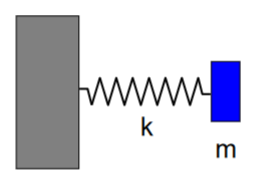
\includegraphics[width=4.5cm]{pictures/Oszillator.png}
    \caption{Oszillator}\label{fig:Oszillator}
\end{wrapfigure}

\[ F = -k\cd x = m\cdot a = m\cdot \ddot{x}\]
DGL lösen dann ist:
\begin{align*}
    x(t) &= x_0 \cdot \cos (w_o\cdot t + \alpha)\\
    v(t) &= -\omega_0 x_0 \sin(\omega_0t+\alpha)\\
    a(t) &= -\omega_0^2 \cos (\omega_0 t + \alpha) = -\omega_0^2 x(t)\\
    & \text{mit: } \omega^2 = \frac{k}{m} \quad \omega = \frac{2\pi}{T} \quad T=2\pi   \cdot \sqrt{\frac{m}{k}}\\
    & \text{komplex:}\\
    x(t)&= A\cdot e^{i(\omega t + \alpha)}\\
    v(t)&= i \cdot \omega \cdot A\cdot e^{i(\omega t + \alpha)} = \omega \cdot A\cdot e^{i(\omega t + \alpha + \frac{\pi}{2})}\qquad (i=e^{i \pi/2}) \\
    a(t)&= -\omega ^2 \cdot A\cdot e^{i(\omega t + \alpha)} = \omega ^2 \cdot A\cdot e^{i(\omega t + \alpha + \pi)}\\
\end{align*}

Die Realteile der komplexen Funktionen liefern die physikalischen Größen zum Zeitpunkt $t$.\\

\subsection{Erzwungene Schwingungen}
$F(t)=F_0\cos (\omega t)$... periodische äußere Kraft, $\omega_0^2=\frac{k}{m}$... Eigenfrequenz des Systems
\begin{align*}
    m\cdot a &= F(t) + F_F = F(t) -k\cdot x\\
    m\cdot \ddot{x} &= F(t) - k\cdot x\\
    \ddot{x}(t)&=\frac{F_0}{m}\cos(\omega t)-\omega_0^2 \cdot x
\end{align*}

\begin{samepage}
    \begin{wrapfigure}{r}{.4\textwidth}
        einsetzen in DGL\\
        $-\omega^2\cdot x_0\cdot e^{i\omega t} = \frac{F_0}{m}\cdot e^{i\omega t} - \omega_0^2 \cdot x_0 \cdot e^{i\omega t}$\\

        $\bm{\Rightarrow x_0=\frac{F_0}{m(\omega_0^2-\omega^2)}}$\\

        \textbf{Resonantzkatastrophe} bei $\omega_0$ da $x_0$ divergiert.
    \end{wrapfigure}
    \textbf{DGL mit komplexen Ansatz lösen:}\\
    \begin{align*}
        F(t) &= F_0\cdot e^{i\omega t}\\
        x(t) &=x_0 \cdot e^{i\omega t}\\
        \dot{x}(t) &= i\cdot \omega \cdot x_0 \cdot e^{i\omega t}\\
        \ddot{x}(t) &= - \omega^2 \cdot x_0 \cdot e^{i\omega t}
    \end{align*}
\end{samepage}



\subsection{Erzwungene, gedämpfte Schwingungen}
\begin{align*}
    m\cdot a &= F(t) + F_F + F_D = F(t) -k\cdot x - d\cdot v\\
    m\cdot \ddot{x} &= F(t) - k\cdot x -d \cdot \dot{x}
\end{align*}




\section{Hydrodynamik}



\subsection{Kontenuitätsgleichung}
Der Volumenstrom in geschlossenen Rohrleitungen ist konstant $Q=const.$.

\subsection{Bernoulli}
In geschlossenen Rohrleitungen ist:\\
$\rho \cdot g\cdot h + \frac{1}{2} \cdot \rho_l \cdot \vec{v}^2 = p + \frac{1}{2} \cdot \rho_l \cdot \vec{v}^2 = const.$\\
konstant.


\subsection{Auftrieb}  
\textbf{Auftriebskraft} greift im Schwerpunkt an.

%%
\subsection{Oberflächenspannung}
\[\bm{\gamma = \frac{\Delta W }{\Delta A}} \quad [\frac{N}{m}]\]\\
$\Delta A$... Vergößerung der Fläche.\\
Je geringer der Durchmesser der Blase, desto höher ist der Druck im Inneren.\\


\section{Thermodynamik}
\subsection{Thermodynamik}

\textbf{Nullter Hauptsatz:} $A=C \wedge B=C \Rightarrow A=B$\\
Befinden sich zwei Systeme A und B jeweils bis Sytem C im Gleichgeweicht, befinden sich auch A und B im Gleichgewicht.\\

$\bm{p \cdot V = const.} \qquad \text{wenn } T=const$. \qquad (Boyle-Mariottesches Gesetz)\\

$\bm{V=V_0+\alpha \cdot T} \text{ für } p=const.$ \qquad (Gay Lussac)\\

1 Torr = 1 mm Hg, 1 bar = $10^5$ Pa [N/mm$^2$], Normaldruck: 1013 mbar = 1013 hPa = 760 Torr\\

Ideale Gasgleichung: $\bm{p\cdot V = N\cdot k_B \cdot T}$\\

Zustandsgleicung: $\bm{p\cdot V = n\cdot R \cdot T}$\\

Extensive Zustandsgrößen: V, N,...\\
(proportional zur Teilchenzahl)\\

Intensive Zustandsgrößen: T, p,...\\

Stoffmenge [mol]: $6,022 \cd 10^{23}$ teilchen/mol = Avogadro Konstante [$N_A$]\\

\section{Arbeit und Energie in der Thermodynamik}
$\bm{dW>0}$ Es wird Energie von außen zugeführt\\

$\bm{dW<0}$ Das System leistet Arbeit\\

\[W=-\int\limits_{V_1}^{V_2}p(V)dV\]

$W$ ist keine \textbf{Zustandsgröße}

\subsection{Wärmefluss}

\textbf{innere Energie U} (ist Zustandsgröße)\\
\[U=\frac{2}{3}k_BNT\]

\subsection{1. Hauptsatz}
 In einem abgeschlossenen System ins die innere Energie U konstant.\\
In einem nicht abgeschlossenen System gilt:
\[\Delta U = W + Q \qquad \text{ mit } W \text{ mechanische Arbeit, }Q\text{ Wärmefluss }\]

\subsection{Wärmekapazität }

\[c_v=\left.\frac{\partial U}{\partial T}\right|_V\]


%%% Verzeichnisse
\newpage
%\listoftables
%\listoffigures
%\printbibliography{}
\end{document}     %%% End the document


